%
%  Created by dariogf on 2006-10-19.
%  Copyright (c) 2006 __MyCompanyName__. All rights reserved.
%

\documentclass[12pt,oneside,a4paper,english]{article}  % (fold)

% Use utf-8 encoding for foreign characters
\usepackage[utf8]{inputenc}
%\usepackage[latin1]{inputenc}

\usepackage[english]{babel} %%%Incluimos el paquete Babel que sirve para separar correctamente las palabras de multitud de idiomas%%%

% Setup for fullpage use
\usepackage{fullpage}

\usepackage{indentfirst}
%\usepackage{pdfsync}

\parskip 3ex % distancia entre los párrafos de texto

% Set dimensions of columns, gap between columns, and paragraph indent 
% \setlength{\textheight}{8.875in}
% \setlength{\textwidth}{6.875in}
% \setlength{\columnsep}{0.3125in}
% \setlength{\topmargin}{0in}
% \setlength{\headheight}{0in}
% \setlength{\headsep}{0in}
% \setlength{\parindent}{3em}
% \setlength{\oddsidemargin}{-.1875in}  % Centers text.
% \setlength{\evensidemargin}{-.1875in}

% Uncomment some of the following if you use the features
%
% Running Headers and footers
%\usepackage{fancyheadings}

% Multipart figures
%\usepackage{subfigure}

% More symbols
\usepackage{amsmath}
%\usepackage{amssymb}
%\usepackage{latexsym}

% Surround parts of graphics with box
\usepackage{boxedminipage}

% Package for including code in the document
\usepackage{listings}
\usepackage{xcolor}

\usepackage{colortbl}

% If you want to generate a toc for each chapter (use with book)
\usepackage{minitoc}

% This is now the recommended way for checking for PDFLaTeX:
\usepackage{ifpdf}

%\newif\ifpdf
%\ifx\pdfoutput\undefined
%\pdffalse % we are not running PDFLaTeX
%\else
%\pdfoutput=1 % we are running PDFLaTeX
%\pdftrue
%\fi

\ifpdf
\usepackage[pdftex]{graphicx}
\else
\usepackage{graphicx}
\fi
\graphicspath{{fotos/}}

\bibliographystyle{plain}

\ifpdf
\DeclareGraphicsExtensions{.pdf, .jpg, .tif}
\else
\DeclareGraphicsExtensions{.eps, .jpg}
\fi


 \title{User manual\\AlignMiner}
 
 \author{Darío Guerrero and 
         Rocío Bautista and 
         M. Gonzalo Claros \\
         Plataforma Andaluza de Bioinformática\\ Universidad de Málaga\\ Severo Ochoa, 34\\ 29590 Málaga, Spain
      }
    
% 
% \date{22-03-2007}

% (end)

\begin{document}
	
%\lstset{language=Java}

\lstset{basicstyle=\scriptsize, commentstyle=\color{blue}}

\maketitle

%\begin{abstract}

%\end{abstract}

%%%%%%%%%%%%%%%%%%%%%%%%%%%%%%%%%%%%%%%%%%%%%%%%%%%%%%%%%%%%%%%%%%%%%
\section{Introduction}\label{sec:introduction} % (fold)
%%%%%%%%%%%%%%%%%%%%%%%%%%%%%%%%%%%%%%%%%%%%%%%%%%%%%%%%%%%%%%%%%%%%%

This document is only a quick guide to AlignMiner, if you need an in-depth explanation you should read the article "XXXXX".

% section introduccion (end)

%\section{Usage}



\subsection{Login in the system}

The first action you need to do in order to use Alignminer is to do a login in the system. Enter any valid email in the form of the main page, as seen in the following picture:

\begin{center}
		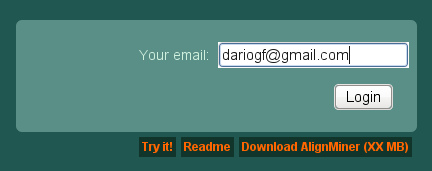
\includegraphics[width=.5\linewidth]{pics/login.jpg}
\end{center}

Once logged in, you can choose between submitting new jobs, or browse already sent ones.

\subsection{Submit a new job}

To submit a new job for execution, you need to upload a file that contains a valid alignment. AlignMiner supports a wide variety of formats (fasta, clustal, msf, ...), so you can try to upload your alignment files without any conversion. Select the alignment to upload using the file field.

You may also provide a name for the job. If not an automatically generated number is assigned.

Click \textbf{send} button to submit the file.

\begin{center}
		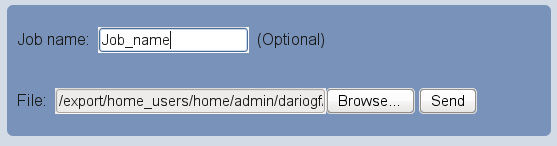
\includegraphics[width=.6\linewidth]{pics/submit.jpg}
\end{center}

When the file has been successfully uploaded to our servers, you will see a new form (and some useful information) where you can select some parameters:

\begin{center}
		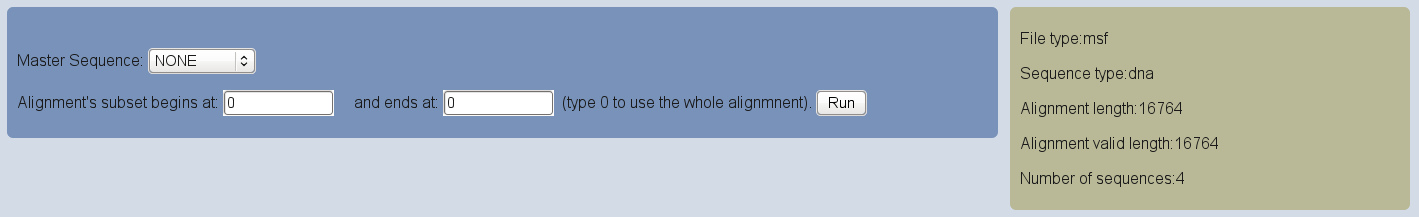
\includegraphics[width=\linewidth]{pics/params.jpg}
\end{center}

\begin{itemize}
\item Master sequence: you can select a master sequence from the popup to be used by scoring methods. If you don't select a master sequence, then a consensus of the whole alignment is calculated.
\item Alignment subset: with this parameter you can force AlignMiner to use only a portion of the alignment. If you leave both fields with zeroes, then an automatic range will be calculated, and weak ends (those with little information) of the alignment will be cropped.
\end{itemize}

Click \textbf{run} when you have modified the desired parameters. You have just sent the job for execution and the job should appear in the job list:

\begin{center}
		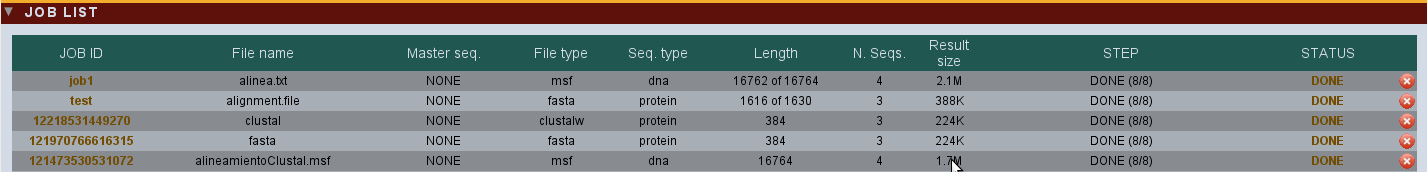
\includegraphics[width=\linewidth]{pics/joblist.jpg}
\end{center}

Actually, the job is run in our supercomputers using a batch queue system, because of that you can view different status of execution in the job list:

\begin{center}
		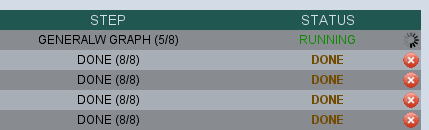
\includegraphics[width=.6\linewidth]{pics/run.jpg}
\end{center}

\begin{itemize}
\item Waiting run: the job has just been uploaded and is waiting you to click the RUN button.
\item Queued: the job has been sent to the batch system and is waiting for resources to be available for execution.
\item Running: the job is running. In the STEP column you can see the completed phases.
\item Done: the job is done and available for browsing.
\item Error: there has been an error that prevents the job from executing correctly. Check the small info icon for more information.
\end{itemize}

Once a job is submitted you can close the system and come later to see its status, or wait it to finish.

\subsection{Browse existing jobs}

Jobs are saved for later browsing, so you can access the system at any time and choose a job from the job list to browse its results.

If you click on a job name, you get a list of available scoring methods:

\begin{center}
		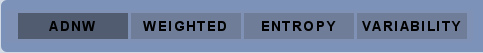
\includegraphics[width=.8\linewidth]{pics/methods.jpg}
\end{center}
		
When a scoring method is selected, a graph is shown with the visual representation of the results. You can drag, zoom or click the graph to your desire:

\begin{center}
		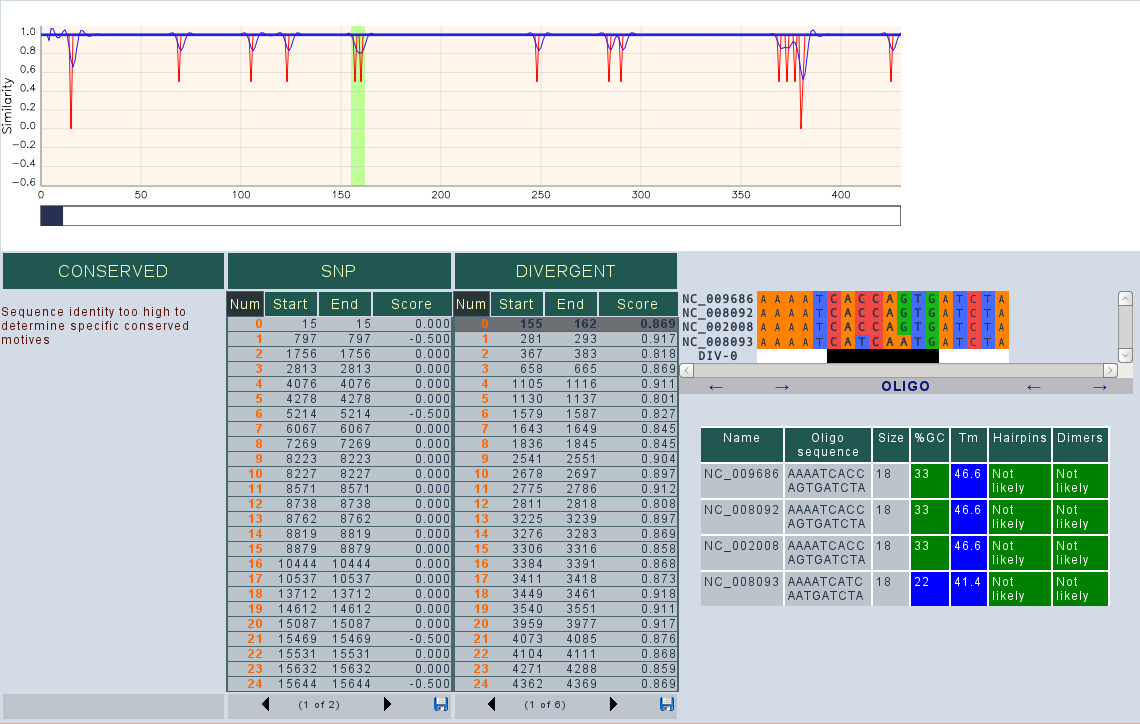
\includegraphics[width=\linewidth]{pics/graph.jpg}
\end{center}

Below the graph, the interesting regions that have been found are presented in tables. You can sort the results by clicking on the column titles. When you click on a row (a region of interest), its corresponding alignment is show at the right of the page. In DNA alignments, characteristics of a putative oligo that uses this region are also calculated. You can change the oligo's width by clicking on the arrows, and its characteristics will be calculated again for you.

% section futuro (end)

% \nocite{MooneySNP}
% \nocite{SNPEST}
% \nocite{MultipleAlign}
% \nocite{LocalWeighting}
%\nocite{ESTprotocol,SNPEST,MooneySNP,EST2uni,ESTpass,LocalWeighting,preAssemble,autoSNP,SNPServer,MultipleAlign}


%\bibliography{bibliografia}

\end{document}
